\documentclass[12pt]{standalone}
\usepackage{tikz}
\usetikzlibrary{arrows.meta}

% Tapered arrow: stacked copies, each thicker and started further along,
% giving a stroke that grows from a thin tail into the head.
% #1 = colour/style, #2 = path.  Taper length fixed at 14pt.
\newcommand{\taperarrow}[2][]{%
  \foreach \i in {1,...,10}{%
    \pgfmathsetmacro{\tw}{1.8*\i/10}%
    \pgfmathsetmacro{\ts}{1.4*(\i-1)}%
    \draw[#1, line width=\tw pt, shorten <=\ts pt,
          line cap=round, rounded corners=4pt] #2;%
  }%
  \draw[#1, line width=1.8pt, shorten <=14pt, rounded corners=4pt,
        -{Stealth[length=8pt,width=7pt]}] #2;%
}
\usetikzlibrary{arrows.meta}

\usepackage{anyfontsize} % allows arbitrary font sizes
\usepackage{lmodern} % better font scaling

\makeatletter
\renewcommand\normalsize{%
  \@setfontsize\normalsize{16pt}{19pt}%
}
\renewcommand\Large{%
  \@setfontsize\Large{20pt}{24pt}%
}
\makeatother

\begin{document}

\begin{tikzpicture}[
  thick, scale=1.2,
  small label/.style={
    anchor=north west,
    font=\scriptsize,
    xshift=-3pt,
    yshift=3pt,
    blue,
    overlay
  }
]
% The query is [3,r]; the band covers it and fades rightwards, stopping at r = 9.
% Fade drawn as flat strips: PDF shadings are dropped by some SVG converters.
\fill[red!17.8, overlay] (2.0000,-0.05) rectangle (2.2504,-4.95);
\fill[red!17.2, overlay] (2.2464,-0.05) rectangle (2.4969,-4.95);
\fill[red!16.8, overlay] (2.4929,-0.05) rectangle (2.7433,-4.95);
\fill[red!16.2, overlay] (2.7393,-0.05) rectangle (2.9897,-4.95);
\fill[red!15.8, overlay] (2.9857,-0.05) rectangle (3.2361,-4.95);
\fill[red!15.2, overlay] (3.2321,-0.05) rectangle (3.4826,-4.95);
\fill[red!14.8, overlay] (3.4786,-0.05) rectangle (3.7290,-4.95);
\fill[red!14.2, overlay] (3.7250,-0.05) rectangle (3.9754,-4.95);
\fill[red!13.8, overlay] (3.9714,-0.05) rectangle (4.2219,-4.95);
\fill[red!13.2, overlay] (4.2179,-0.05) rectangle (4.4683,-4.95);
\fill[red!12.8, overlay] (4.4643,-0.05) rectangle (4.7147,-4.95);
\fill[red!12.2, overlay] (4.7107,-0.05) rectangle (4.9611,-4.95);
\fill[red!11.8, overlay] (4.9571,-0.05) rectangle (5.2076,-4.95);
\fill[red!11.2, overlay] (5.2036,-0.05) rectangle (5.4540,-4.95);
\fill[red!10.8, overlay] (5.4500,-0.05) rectangle (5.7004,-4.95);
\fill[red!10.2, overlay] (5.6964,-0.05) rectangle (5.9469,-4.95);
\fill[red!9.8, overlay] (5.9429,-0.05) rectangle (6.1933,-4.95);
\fill[red!9.2, overlay] (6.1893,-0.05) rectangle (6.4397,-4.95);
\fill[red!8.8, overlay] (6.4357,-0.05) rectangle (6.6861,-4.95);
\fill[red!8.2, overlay] (6.6821,-0.05) rectangle (6.9326,-4.95);
\fill[red!7.8, overlay] (6.9286,-0.05) rectangle (7.1790,-4.95);
\fill[red!7.2, overlay] (7.1750,-0.05) rectangle (7.4254,-4.95);
\fill[red!6.8, overlay] (7.4214,-0.05) rectangle (7.6719,-4.95);
\fill[red!6.2, overlay] (7.6679,-0.05) rectangle (7.9183,-4.95);
\fill[red!5.8, overlay] (7.9143,-0.05) rectangle (8.1647,-4.95);
\fill[red!5.2, overlay] (8.1607,-0.05) rectangle (8.4111,-4.95);
\fill[red!4.8, overlay] (8.4071,-0.05) rectangle (8.6576,-4.95);
\fill[red!4.2, overlay] (8.6536,-0.05) rectangle (8.9040,-4.95);
% Layer 1.
\draw (0,0) node[small label] {1} rectangle (12.9,-0.9);
\node at (6.45,-0.45) {$[1,13]$};
% Layer 2.
\draw (0,-1) node[small label] {2} rectangle (6.9,-1.9);
\node at (3.45,-1.45) {$[1,7]$};
\draw[ultra thick, densely dashed] (7,-1) node[small label] {15} rectangle (12.9,-1.9);
\node at (9.95,-1.45) {$[8,13]$};
% Layer 3.
\draw (0,-2) node[small label] {3} rectangle (3.9,-2.9);
\node at (1.95,-2.45) {$[1,4]$};
\draw[ultra thick] (4,-2) node[small label] {10} rectangle (6.9,-2.9);
\node at (5.45,-2.45) {$[5,7]$};
\draw[ultra thick, densely dashed] (7,-2) node[small label] {16} rectangle (9.9,-2.9);
\node at (8.45,-2.45) {$[8,10]$};
\draw (10,-2) node[small label] {21} rectangle (12.9,-2.9);
\node at (11.45,-2.45) {$[11,13]$};
% Layer 4.
\draw (0,-3) node[small label] {4} rectangle (1.9,-3.9);
\node at (0.95,-3.45) {$[1,2]$};
\draw[ultra thick] (2,-3) node[small label] {7} rectangle (3.9,-3.9);
\node at (2.95,-3.45) {$[3,4]$};
\draw (4,-3) node[small label] {11} rectangle (5.9,-3.9);
\node at (4.95,-3.45) {$[5,6]$};
\draw (6,-3) node[small label] {14} rectangle (6.9,-3.9);
\node at (6.45,-3.45) {$7$};
\draw[ultra thick] (7,-3) node[small label] {17} rectangle (8.9,-3.9);
\node at (7.95,-3.45) {$[8,9]$};
\draw[ultra thick, densely dashed] (9,-3) node[small label] {20} rectangle (9.9,-3.9);
\node at (9.45,-3.45) {$10$};
\draw (10,-3) node[small label] {22} rectangle (11.9,-3.9);
\node at (10.95,-3.45) {$[11,12]$};
\draw (12,-3) node[small label] {25} rectangle (12.9,-3.9);
\node at (12.45,-3.45) {$13$};
% Layer 5.
\draw (0,-4) node[small label] {5} rectangle (0.9,-4.9);
\node at (0.45,-4.45) {$1$};
\draw (1,-4) node[small label] {6} rectangle (1.9,-4.9);
\node at (1.45,-4.45) {$2$};
\draw (2,-4) node[small label] {8} rectangle (2.9,-4.9);
\node at (2.45,-4.45) {$3$};
\draw (3,-4) node[small label] {9} rectangle (3.9,-4.9);
\node at (3.45,-4.45) {$4$};
\draw (4,-4) node[small label] {12} rectangle (4.9,-4.9);
\node at (4.45,-4.45) {$5$};
\draw (5,-4) node[small label] {13} rectangle (5.9,-4.9);
\node at (5.45,-4.45) {$6$};
\draw (7,-4) node[small label] {18} rectangle (7.9,-4.9);
\node at (7.45,-4.45) {$8$};
\draw (8,-4) node[small label] {19} rectangle (8.9,-4.9);
\node at (8.45,-4.45) {$9$};
\draw (10,-4) node[small label] {23} rectangle (10.9,-4.9);
\node at (10.45,-4.45) {$11$};
\draw (11,-4) node[small label] {24} rectangle (11.9,-4.9);
\node at (11.45,-4.45) {$12$};
% The query starts at l and extends rightwards as far as the condition allows.
\draw[red!75!black, line width=1.2pt] (2.0,0.16) -- (2.0,0.40);
\draw[red!75!black, line width=1.2pt, -{Stealth[length=7pt,width=6pt]}]
  (2.0,0.28) -- (8.9,0.28);
\node[red!75!black, anchor=south] at (2.0,0.44) {$l=3$};
\node[red!75!black, anchor=south] at (8.9,0.44) {$r$};
% Each fork starts at the node's own split point and enters both children.
% [1,13] splits at 7: into [1,7] and [8,13].
\taperarrow[red!75!black]{(6.95,-0.80) -- (6.00,-1.28)}
\taperarrow[red!75!black]{(6.95,-0.80) -- (7.95,-1.28)}
% [1,7] splits at 4: into [1,4] and [5,7].
\taperarrow[red!75!black]{(3.95,-1.80) -- (3.05,-2.28)}
\taperarrow[red!75!black]{(3.95,-1.80) -- (4.60,-2.28)}
% [1,4] splits at 2: into [1,2] and [3,4].
\taperarrow[red!75!black]{(1.95,-2.80) -- (1.62,-3.28)}
\taperarrow[red!75!black]{(1.95,-2.80) -- (2.25,-3.28)}
% [8,13] descends only into [8,10]; its right child is never reached.
\taperarrow[red!75!black]{(9.15,-1.80) -- (9.15,-2.28)}
% [8,10] splits at 9: into [8,9] and [10,10].
\taperarrow[red!75!black]{(8.95,-2.80) -- (8.70,-3.28)}
\taperarrow[red!75!black]{(8.95,-2.80) -- (9.20,-3.28)}
\end{tikzpicture}

\end{document}
